\documentclass[a4paper,10pt]{article}\large
\usepackage{iplouccfg}
\usepackage{zhfontcfg}

\linespread{1.5}\selectfont
\pagestyle{fancy}
\lhead{}
\chead{}
\chead{视觉神经传导通路综述}
\rhead{}
\lfoot{中国海洋大学}
\cfoot{赵红苗}
\rfoot{\thepage}
\renewcommand{\headrulewidth}{0.4pt}
\renewcommand{\footrulewidth}{0.4pt}
\setlength{\parindent}{2em} 
%opening
\title{视觉神经传导通路}
\author{赵红苗}
\date{2013年7月2日}
\begin{document}
\maketitle

\begin{abstract} 
视觉是人类最重要的感觉,人类70\%以上的信息来自视觉系统,视觉研究是神经科学发展最快的领域之一。视觉神经传导是神经系统传导的一个重要组成部分,它使生物体具有视知觉能力,它使用可见光信息构筑机体对周围世界进行感知。经过漫长的进化,人类的视觉系统已经达到高度完美的阶段。本文的主要目的是通过介绍视觉神经传导通路对视觉传导机制和认知有更深入的认识,从而在今后对视觉注意的生物学模型的建模有更好的理解。本文将从神经学和解剖学的角度来介绍视觉神经传导通路。


\begin{description}
\item[关键词:视觉,  视觉系统,  视觉神经传导通路,  认知,  解剖学, 神经学]
\end{description}
\end{abstract}

\newpage
\tableofcontents 
\newpage
\section{引言}
\subsection{研究背景}
2013年4月2日,奥巴马宣布投入巨资启动“脑计划”\cite{1:misc},这是继人类基因组计划之后的又一针对人类自身难题的重大研究计划。该计划旨在通过创新的神经技术加强对人脑的认识。脑与认知\cite{6:article}所涉及的面非常广,包括神经生物学、解剖学、心理学、计算机科学、分子生物学等,是多交叉的学科。视觉研究是探索脑功能的一个重要研究领域,视觉研究也是认识人脑信息处理加工、学习记忆、抽象思维等高级脑功能的重要途径。外部世界是丰富多彩、永远变化和运动的,因此对视知觉的研究已成为认知神经科学的热门课题之一。


现在,视知觉的研究中已取得了一系列成果\cite{3:misc}:在视网膜的光感受器水平已克隆出视色素蛋白基因,通过光感受器细胞膜超极化,使得光能就转化为神经电信号;在视网膜,发现这个两维的、多层次信息处理的最后结果,是经由视网膜神经节细胞以动作电位脉冲调频的方式,传递给脑的;在感受野部分,视通路中任一神经元都在视网膜(或视野)上有一个代表区域即同心圆拮抗型感受野;在初级视觉皮层发现了功能柱,其柱内细胞具有相同的最优方位、相同的眼优势、相同的最优空间频率。


\subsection{视觉神经传导通路}
视觉神经传导通路是视觉信息加工和处理的神经路线,外界的物体在视网膜成像时,实际上是光线这个刺激因素被视网膜的感光细胞(视杆细胞和视锥细胞)转变为电信号,后者经视网膜内双极细胞传到神经节细胞形成神经冲动,即视觉信息。视觉信息再经视神经传向脑。


视觉传导通路由3级神经元组成\cite{4:misc}。第l级神经元为视网膜的双极细胞,其周围支与形成视觉感受器的视锥细胞和视杆细胞形成突触,中枢支与节细胞形成突触。第2级神经元是节细胞,其轴突在视神经盘(乳头)处集合向后穿巩膜形成视神经。视神经向后经视神经管入颅腔,形成视交叉后,延为视束。在视交叉中,只有一部分纤维交叉,即来自两眼视网膜鼻侧半的纤维交叉,走在对侧视束中;颞侧半的不交叉,走在同侧视束中。因此,左侧视束含有来自两眼视网膜左侧半的纤维,右侧视束含有来自两眼视网膜右侧半的纤维。视束行向后外,绕大脑脚,多数纤维止于外侧膝状体。第3级神经元的胞体在外侧膝状体内,它们发出的大量纤维组成所谓的视辐射,视辐射的纤维最后投射到大脑枕叶的视觉中枢-即视皮质。视觉信息只有传到脑的视皮质并经过处理、分析,才能最后形成主观的视觉感受。图\ref{fig 1}表示视觉传输的整个通路。


\begin{figure}[!htb]
\centering
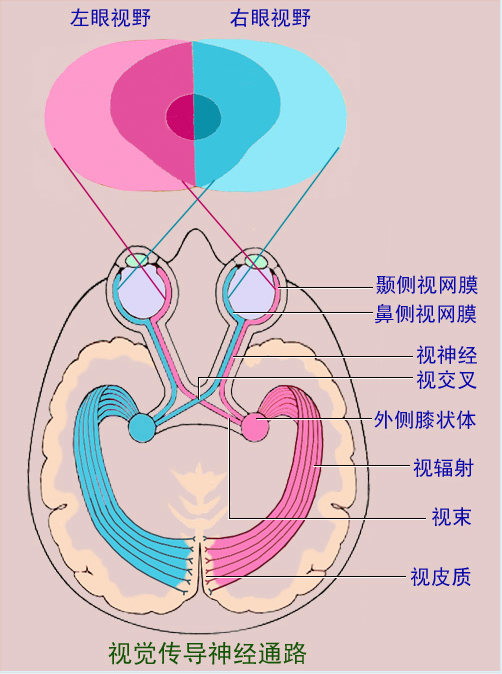
\includegraphics[width=0.5\textwidth]{shijuexitong.png}
\caption{视觉传导神经通路}\label{fig 1} 
\end{figure}


\subsection{本文主要工作与安排}

本文主要针对视觉神经传导通路进行详细介绍,重点介绍视觉神经传导各部分所起的作用。本文的主要安排如下:


第一部分对视觉神经传导通路的的研究背景及研究状况进行了介绍,并对全文的主要工作即安排作了说明;


第二部分主要介绍神经元的结构、分类、如何进行信息的传递及作用,这是视觉传输的基础;


第三部分介绍了视觉信息处理的初级部分---视网膜,对视网膜的组成、各部分的特点及作用进行详细介绍;


第四部分介绍了视觉信息处理的中间环节---外侧膝状体,并对外侧膝状体的结构、特点及功能进行详细介绍;


第五部分介绍了视觉信息处理的高级区域---视皮层,对视皮层的组成、各部分的特点及作用进行论文详细的介绍;


第六部分总体归纳了整个视觉传导的神经通路,对视觉神经通路进一步解析,是全文的重点;


第七部分是全文的总结,回顾所做的工作,展望以后的工作方向。

\section{神经元} 

\subsection{神经元结构}

\begin{figure}[htb]
\centering

\par \hspace{2ex}
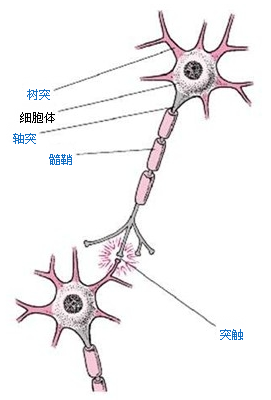
\includegraphics[width=0.5\textwidth]{NerveCell.png}
\caption{神经元}\label{fig 2} 
\end{figure}


神经元\cite{18:book}如图\ref{fig 2},又名神经原或神经细胞,是神经神经系统的结构与功能单位之一(占了神经系统约10\%,其他大部分由胶状细胞所构成)。虽然神经元形态与功能多种多样,但结构上大致都可分成胞体和神经突两部分。神经突又分树突和轴突两种。轴突往往很长,由细胞的轴丘分出,其直径均匀,开始一段称为始段,离开细胞体若干距离后始获得髓鞘,成为神经纤维。习惯上把神经纤维分为有髓纤维与无髓纤维两种,实际上所谓无髓纤维也有一薄层髓鞘,并非完全无髓鞘。胞体的大小差异很大,小的直径仅5$\sim$6μm,大的可达100μm以上。突起的形态、数量和长短也很不相同。树突多呈树状分支,它可接受刺激并将冲动传向胞体;轴突呈细索状,末端常有分支,称轴突终末,轴突将冲动从胞体传向终末。通常一个神经元有一个至多个树突,但轴突只有一条。神经元的胞体越大,其轴突越长。

\subsection{神经元分类}

神经元的分类有多种方法,常以神经元突起的数目、功能以及所释放的递质进行分类。

\subsubsection{根据神经元突起的数目分类}

 
假单极神经元:从胞体发出一个突起,在离胞体不远处呈T型分为两支,因此,称假单极神经元。其中一支突起细长,结构与轴突相同,伸向周围,称周围突,其功能相当于树突,能感受刺激并将冲动传向胞体;另一分支伸向中枢,称中枢突,将冲动传给另一个神经元,相当于轴突。如脊神经节内的感觉神经元等。


双极神经元:从胞体两端各发出一个突起,一个是树突,另一个是轴突。如耳蜗神经节内的感觉神经元等。


多极神经元:有一个轴突和多个树突,是人体中数量最多的一种神经元,如脊髓前角运动神经元和大脑皮质的锥体细胞等。多极神经元又可依轴突的长短和分支情况分为两型:(1)高尔基Ⅰ型神经元,其胞体大,轴突长,在行径途中发出侧支,如脊髓前角运动神经元;(2)高尔基Ⅱ型神经元,其胞体小,轴突短,在胞体附近发出例支,如脊髓后角的小神经元以及大、小脑内的联合神经元。


\subsubsection{根据神经元的功能分类}

感觉神经元:也称传入神经元是传导感觉冲动的,胞体在脑、脊神经节内,多为假单极神经元。其突起构成周围神经的传入神经。神经纤维终末在皮肤和肌肉等部位形成感受器。


运动神经元:也称传出神经元,是传导运动冲动的神经元,多为多极神经元。胞体位于中枢神经系统的灰质和植物神经节内,其突起构成传出神经纤维。神经纤维终未,分布在肌组织和腺体,形成效应器。


中间神经元:也称联合神经元是在神经元之间起联络作用的神经元,是多极神经元,人类神经系统中,最多的神经元,构成中枢神经系统内的复杂网络。胞体位于中枢神经系统的灰质内,其突起一般也位于灰质。


\subsubsection{根据神经元释放的递质分类}

胆碱能神经元:该神经元的神经末梢能释放乙酸胆碱,如脊髓前角运动神经元等。


胺能神经元:能释放单胺类神经递质:肾上腺素、去甲肾上腺素、多巴胺、5-羟色胺、组胺等。如能释放肾上腺素的称为肾上腺素能神经元,如交感神经节内的神经元等。


氨基酸能神经元:能释放谷氨酸、氨基丁酸等。


肽能神经元:能释放脑啡肽、P物质等肽类物质,如下丘脑和肌间神经丛内的一些神经元等。这类神经元所释放的物质总称为神经肽。有观点认为神经肽不直接引起效应细胞的改变,仅对神经递质的效应起调节作用,故将神经肽称为神经调质。

\subsubsection{神经元分布}

神经元的细胞体主要分布脑和脊髓里,这里集中密集的地方,色泽灰暗,叫做灰质。在灰质里,功能相同的神经细胞体汇集在一起,调节人体的某一项相应的生理活动,这部分结构就叫做神经中枢。在周围神经系统里,也有一些由功能相同的神经元细胞体汇集在一起,这部分结构叫做神经节。


神经元的神经纤维主要集中在周围神经系统里。在周围神经系统里,许多神经纤维集结成束,外面包着结缔组织形成的膜,就成为一条神经。在脑和脊髓里,也有神经纤维分布,他们密集的部位,色泽亮白,叫做白质。白质内的神经纤维,有的能向上传导兴奋,有的能向下传导兴奋。


\subsection{信息在神经元间传递}


神经元最主要的功能是通过突触进行细胞间的信息传递。突触是两个神经元之间或神经元与效应器细胞之间相互接触、并借以传递信息的部位,突触也是一种细胞连接方式,最常见的是一个神经元的轴突终末与另一个神经元的树突、树突棘或胞体连接,分别形成轴-树突触、轴-棘突触或轴-体突触。突触有电突触和化学性突触,但以化学性突触为主。电突触通过缝隙连接直接完成细胞间的电信息传递,化学性突触传递必须依赖于神经递质或神经肽作用于突触后膜的受体而完成细胞间的信息传递。图\ref{fig 3}是突触的结构:

\begin{figure}[htb]
\centering

\par \hspace{2ex}
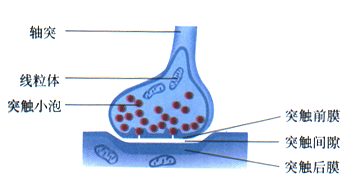
\includegraphics[width=0.7\textwidth]{TuChu.png}
\caption{突触}\label{fig 3} 
\end{figure}

电镜下,突触由突触前膜,突触间隙和突触后膜三部分构成。突触前、后成分彼此相对的胞膜,分别称突触前膜和突触后膜,两者之间有宽15$\sim$30nm的突触间隙。突触前成分一般是神经元的轴突终末,呈球状膨大,在银染的光镜标本中呈现为棕黑色的圆形颗粒,称突触小体。突触前成分(或突触小体)内含许多突触小泡。突触小泡内含神经递质或神经调质。突触前、后膜均较一般细胞膜略厚,乃因突触前、后膜胞质面有一些致密物质附着。


当神经冲动沿轴膜传导到轴突终末时,突触小泡脱离细胞骨架,移至突触前膜并与之融合,通过出胞作用释放小泡内容物到突触间隙。突触后膜中的受体与特异性神经递质结合后,膜内离子通道开放,改变突触后膜两侧的离子分布,使突触后神经元(或效应细胞)出现兴奋性或抑制性突触后电位。


由于突触的单向传递,中枢神经系统内冲动的传递就有一定的方向,即由传入神经元传向中间神经元,再传向传出神经元,从而使整个神经系统的活动能够有规律地进行。


\section{眼睛}

\begin{figure}[htb]
\centering

\par \hspace{2ex}
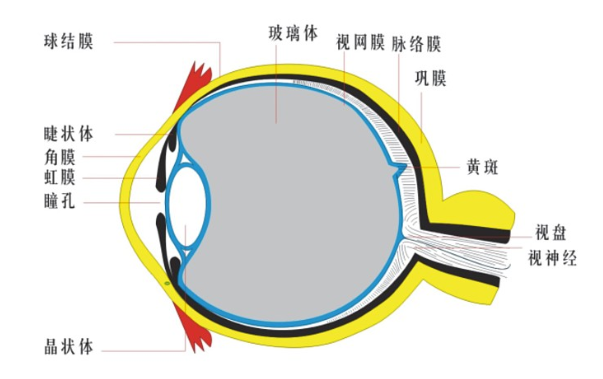
\includegraphics[width=0.7\textwidth]{Eye.png}
\caption{眼睛结构}\label{fig 4} 
\end{figure}

眼睛\cite{11:misc}的一般结构如图\ref{fig 4},人的眼睛是一个近似球体,直径约23mm,由眼球和眼球壁构成。眼球壁分为三层,最外层的正前方占据了1/6 面积的是一层弹性的透明组织,叫做角膜,具有屈光作用,光线经过角膜发生曲折进入眼内。其余的5/6是白色的巩膜,主要起到保护眼球的作用。眼球壁的中层包括虹膜、睫状体和脉络膜。角膜的后面、晶状体的前面是虹膜,虹膜中央的圆孔称为瞳孔,虹膜的肌肉组织可以调节瞳孔的大小。睫状体在虹膜后面,其中的睫状肌可以调节晶状体的曲率半径。脉络膜呈黑色,隔绝外部光线,并且消除光线在眼球内部的乱反射,使得眼球内部成为暗箱。眼球壁的内层是视网膜,厚度约0.5mm左右。视觉信息从这里开始第一步处理,从光信号转化为生物电信号\cite{16:book}。


视网膜实际上是脑及其微小的一部分\cite{15:book},在早期发育中它就从大脑中分离出来,但通过视神经束与大脑保持着适当的联系。其厚度只有0.1mm—0.5mm,但结构及其复杂,视网膜从外到内主要分为三层结构:光感受器层、双极细胞层以及神经节细胞层。在这三层之间存在着相互联系的水平细胞和无足细胞,起到综合和相互通信的作用。视网膜的结构如图\ref{fig 5}所示:

\begin{figure}[htb]
\centering
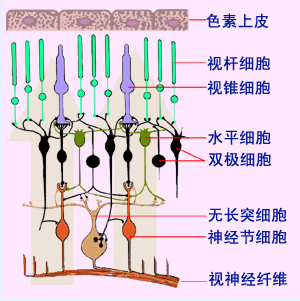
\includegraphics[width=0.5\textwidth]{shiwangmo.png}
\caption{视网膜结构}\label{fig 5} 
\end{figure}


每个视网膜约有12亿个光感受器\cite{15:book},在光感受器层有两类感受器细胞:视杆细胞与视锥细胞。在视网膜中者来嗯中细胞分布极不均匀。视杆细胞数量超过十亿,形状细而长,能感受其极微弱的光线,并且仅有一种类型。一个光量子就可以引起一个视杆细胞兴奋,5个光量子就能使人眼感觉到一个闪光,但视杆细胞不能分辨颜色。视锥细胞得到数目约有七百万,形状粗而短,强光刺激才能引起兴奋,但具有颜色分辨能力。目前普遍认为视网膜中存在三种不同的视锥细胞\cite{17:book},它们光谱吸收曲线的峰值波长分别为560nm、530nm以及430nm,对红、绿、蓝三种颜色最为敏感,因此我们可以看到不同的颜色。


视杆细胞和视锥细胞在形态上\cite{11:misc}都可分为四部分,有外向内依次称为外段、内断、胞体和终足。外段是视色素集中的部位,在感光换能中其重要作用。视杆和视锥细胞在形态上的区别,也主要在于外段的不同。视杆细胞和视锥细胞外段内含很多个重叠成层排列整齐的圆盘状结构—膜盘。膜盘就像一个扁平的囊,它的表面膜上镶嵌着蛋白质,这些蛋白质绝大部分是一种被称为视紫红质的视色素。人的每个视杆细胞的外段中有近千个膜盘,每个膜盘所含的视紫红质分子约一百万个。


感受器细胞在视网膜上的分布是不均匀的\cite{15:book}。在视网膜的中心有一个直径约1.5mm的区域称为黄斑\cite{11:misc},黄斑中心的凹陷称为中央凹,中央凹是视觉最敏锐的地方。在中央凹区域,没有视杆细胞,只有视锥细胞,并且视锥细胞的密度高达每平方毫米150000个左右。这里锥细胞与双极细胞是一对一的连接,因而视觉最为敏锐精确。从中央凹向外延伸,视锥细胞的密度迅速降低,至80°左右彻底消失。而视杆细胞的密度在中央凹以外$15\,^{\circ}$-$30\,^{\circ}$的区域最大。视网膜的这种生理结构特点决定了眼睛的分辨能力是不均匀的,它保证了人眼对感兴趣区域的高分辨率,同时压缩周边的信息。


在光感受器细胞与双极细胞之间链接着水平层细胞,双极细胞接收光感受器和水平细胞的信号输入\cite{5:article},在整合后传递至无长突细胞和神经节细胞。水平细胞对刺激的反应相对较慢,当光感受器检测到运动的目标时,水平细胞依然记录着目标运动前位置的信息。双极细胞的输出电位正比于光感细胞与水平细胞差值的对数,因此,双极细胞的输出包含了对于运动检测的重要信息。


把信号从眼睛送达大脑的细胞叫神经节细胞\cite{15:book},它位于视网膜最终段,在视网膜中约有一百万个。神经节细胞由多极的节细胞组成,其树突主要与双极细胞联系,也可通过无足细胞横向联系;其轴突延伸至视神经乳头处,穿过筛板,形成视神经,由眼球出来之后,经过视束交叉,形成视束,止于外侧膝状体。神经节细胞根据对感受野的响应不同大致可分为两种细胞:ON型细胞和OFF型细胞\cite{5:article}。一个神经元所响应的刺激区域称作该神经元的感受野。在视觉系统中,光感受器将光信号转换为电信号,通过视觉通路传递至许多神经细胞;反过来看,每个神经细胞的输入都直接或间接来自一部分光感受器,这部分光感受器就是该神经细胞的感受野。神经节细胞的感受野是同心圆的结构\cite{17:book},呈现出独特的中央-周围拮抗性质。研究表明同心圆拮抗式感受野的数学模型可用高斯分布来表示,即高斯差模型。若中央为兴奋区域,周围为抑制区域,称为ON型感受野;反之,若中央为抑制区域,周围为兴奋区域,称为OFF型感受野。


如图\ref{fig 6}所示,当小光斑照射中心区域时,On型感受野开始兴奋,而且兴奋强度随着光斑面积的增加而增加,当光斑正好覆盖全部中央区域时兴奋最强烈;而Off型感受野一直处于抑制状态。当光斑仅照射周围区域时,Off型感受野开始兴奋,而且兴奋强度随着光斑面积的增加而增加,当光斑正好覆盖全部周围区域时兴奋最强烈;而On型感受野一直处于抑制状态。当光斑面积进一步加大,覆盖整个感受野时,兴奋区域与抑制区域相互抵消,只得到较弱的反应。换句话说,感受野中心区域的响应与周边是相反的\cite{16:book}。这意味着任何一个特定的神经节细胞对在恰当位置上的光点刺激具有强脉冲兴奋,而对其整个区域的均匀光刺激并没有响应。视网膜就是要去掉部分传入眼睛里的冗余信息。它传送到脑中的正是在视野中的感兴趣的信息,在那里光分布是不均匀的,而要忽略忽的正是几乎不变的部分。

\begin{figure}[htb]
\centering
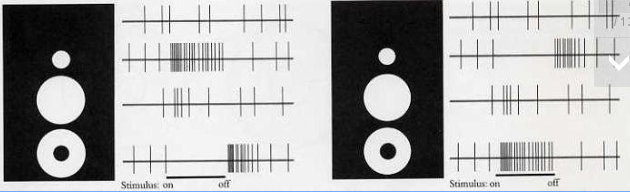
\includegraphics[width=0.6\textwidth]{ganshouye.png}
\caption{感受野分布}\label{fig 6} 
\end{figure}


神经节细胞主要包括M细胞(M细胞是指Magno,意思为大)和P细胞(P细胞是指Parvo,意思是小)\cite{16:book},每一类都具有ON型中心的感受野和OFF型中心的感受野。在视网膜的任何地方,M细胞都比P细胞大,而且也具有大的感受野。他们还有粗厚的轴突,这就使这就信号的传导速度加快。同时,M细胞对光强分布中的微小差别敏感,因此它能很好处理低对比度,但是它们的发射率在高对比度时达到饱和。它们主要用于对视觉中的场景变化发出信号。P细胞更多,与M细胞相比,它们的反映具有更好的线性,即正比于输入,而且它们对于颜色、细节、高反差和颜色更感兴趣。总结起来,大细胞具有检测运动和闪烁目标的作用,小细胞可以分辨颜色、纹理、形状和视差。


基于视觉系统的视觉信号传输到大脑,视网膜被垂直的分成两个部分,颞测(靠近颞的一侧)和鼻侧(靠近鼻的一侧)。颞侧的一半视神经纤维投射到同侧,鼻侧的一半视神经纤维投射到对侧。最终使得右侧的视觉信息投射到左脑,左侧的视觉信息投射到右脑。

\section{外侧膝状体}

外侧膝状体是视觉通路上传递信息不可或缺的中间环节\cite{5:article},属于丘脑的一部分,其形状如图\ref{fig 7}所示。来自不同眼球的视神经在视交叉处交汇并根据视野进行划分,右侧视野的信息在左视束中传递,左侧视野的信息在右视束中传递,这样单侧外膝状体得到的是双眼输入的对侧视野内的视觉信息。然后外侧膝状体再将信息传递至大脑皮层,这段通路上再没有其他神经元。

\begin{figure}[htb]
\centering
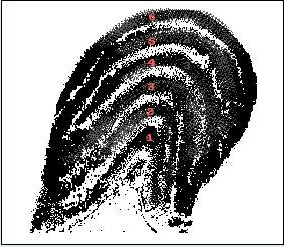
\includegraphics[width=0.6\textwidth]{waixiti.png}
\caption{外侧膝状体}\label{fig 7} 
\end{figure}


视网膜中90\%的输出都传递至外侧膝状体,但这些仅占到外侧膝状体所有输入20\%,其他大部分输入来自于大脑皮层的反馈连接\cite{13:misc}。人类的外侧膝状体有6层,其中1、4、6层接收的是一只眼睛的信息,而2、3、5层接收的是另一只眼睛的信息,它们之间几乎没有相互作用,其接受信息如图\ref{fig 8}所示。1、2层的细胞为大细胞层,对颜色无选择性,空间分辨率较低,而对比敏感度高;4、6、3、5层的细胞为小细胞层,对颜色有选择性,空间分辨率高,而对比敏感度较低。这样,不同的视觉信息已经明显的被分开,并且由不同类型的细胞进行并行处理。视网膜神经节细胞投射到外膝状体核各层时是极有规律的,将外膝状体各层接收投射的响应细胞部位连接起来,就会得到大体上与各层边界垂直的线,称作投射线。通常认为外侧膝状体综合了双眼的各种信息,包括空间频率、颜色以及视差等等,而且其感受野与视网膜节细胞的感受也非常相似,都是中央-周围拮抗的同心圆模式,也分为On型感受野与Off型感受野。到目前为止,外侧膝状体的具体功能还是未知的。

\begin{figure}[htb]
\centering
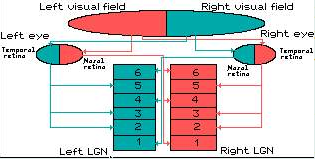
\includegraphics[width=0.5\textwidth]{waixitijieshouxinxi.png}
\caption{外侧膝状体接收信息示意图}\label{fig 8} 
\end{figure}

\section{视觉皮层}


视觉皮层是大脑皮层中主要负责处理视觉信息的部位,位于大脑后部的枕叶,是一种典型的感觉型粒状皮层。在一起大约占大脑皮层总面积的55\%左右,这也从侧面反映了处理视觉信息是大脑的一个非常重要的功能。人类的视觉皮层\cite{15:book}包括初级视皮层(V1,亦称纹状皮层)以及纹外皮层(V2,V3,V4,V5等)。初级视皮层位于Brodmann17区,纹外皮层包括Brodmann18区和Brodmann19区。大脑的两个半球各有一部分视觉皮层。左半球的视觉皮层从右视野接收信息,而右半球的视觉皮层从左视野接收信息\cite{12:book}。


上世纪60年代,Hubel和Wiesel首次研究视皮层细胞对光刺激的反映时,意外地发现\cite{16:book}这些细胞都有共同的特点,即对大面积弥散光刺激没有反应,而对有一定方位或朝向的亮暗对比边或光棒、暗棒有强烈反应,若该刺激物的方位偏离该细胞“偏爱”的最优方位,细胞反应便停止或骤减,因此强烈的方位选择性是绝大多数视觉皮层细胞的共性。


初级视皮层(V1)的输出信息出送到两个渠道\cite{6:article},分别成为背侧流(Dorsal stream)和腹侧流(Ventral stream)。背侧视觉信息流通路从V1出发经过V2,进入背内侧区和中颞区(MT,亦称V5),然后抵达顶下小叶,常被称为空间通路,参与处理物体的空间位置信息以及相关的运动控制; 腹侧视觉信息流通路起始于V1,经过V2和V4到达下颞叶,常被称为内容通路,这条通路负责分析形状、轮廓、颜色,并检测和辨认物体。背侧流和腹侧流也常常被称为what通路和where通路\cite{15:book}。


\subsection{V1视皮层}


V1区\cite{16:book}是视觉皮层中第一个进行视觉处理的区域,即大脑皮层17区或视觉初级皮层,是大脑皮层中被研究得最透彻的区域。一个半球中V1的大小和厚度与一张信用卡相仿,人类的V1很大一部分隐藏在脑内壁的距状裂中。V1区相当大,每平方毫米表面下有将近25万个神经元\cite{8:article}。LGN的输出,即多达几百万根的膝状体轴突投射到V1的不同亚层,具体投射到哪个亚层取决于LGN的中继细胞是从哪类视网膜神经节细胞接受的输入。


V1层状结构为了描述方便,可以将其分为六层\cite{15:book},实际上在层中还包含有几个亚层。最外面的一层为第一层,它具有很少的细胞体,主要是由位于它下面层中的锥体细胞向上延伸形成的树突末梢间的相互连接的轴突构成。因此,它都是这些神经布线而很少有细胞体。在它的下面是2、3层,常常统称之为上层。在这些层中有许多锥体细胞。第四层是由许多兴奋型的星状细胞构成,而几乎没有锥体细胞。第5、6层称为下层,它包含有许多锥体细胞,其中一些细胞树突末梢一直可达到第一层。


信息究竟在皮层的各层之间是怎样传递的,这是个复杂的问题。进入皮层区的主要的,但不是唯一的入口位于它的第四层\cite{16:book}。 第四层主要连接到上不的第2、3层,然后,又依次与第五层形成一个很大的局域连接,一直到达位于它下面的第六层。第六层又依次通过短的垂直联系返回到第四层。第一层还接收来自其他皮层的一些主要的输入。这些与来自低层的高锥体细胞的树突末梢相联系。示意图如图\ref{fig 9}所示:


\begin{figure}[htb]
\centering
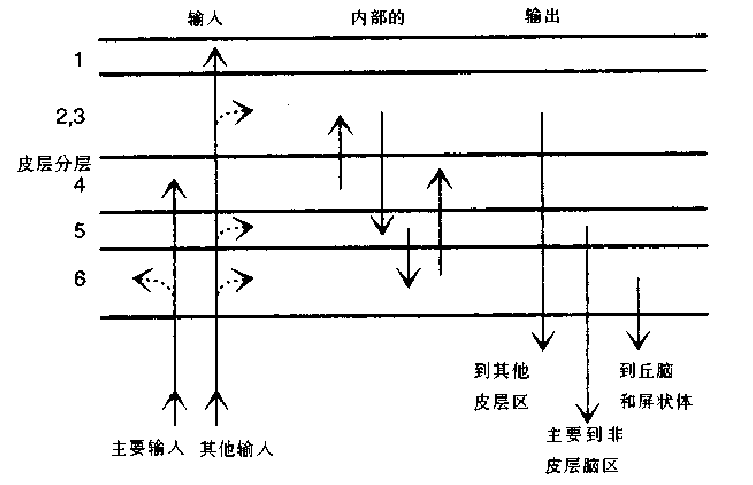
\includegraphics[width=0.7\textwidth]{V1chuanshu.png}
\caption{皮层内部的信息传输}\label{fig 9} 
\end{figure}


V1中的绝大多数细胞对边缘、条形物或光栅刺激能产生反应\cite{15:book}。一些细胞对特定朝向的亮条有反应,一些则偏好在明亮背景之上具有相同朝向的暗条,还有一些则对明暗边缘有较强反应。


\subsection{V2视皮层}



V2视皮层\cite{9:article}在结构上紧紧围绕初级视皮层皮层,主要接收来自V1皮层的前馈信息投射,并且向V1皮层发出几乎等量的反馈投射。V2是皮层信息传递通路的第二站,几乎所有从V1皮层传出的信息都要经过V2皮层,然后传送到V3、V4、MT等纹外皮层区域。除了大量接收初级视皮层的信息输入之外,V2皮层还接收丘脑枕的前馈投射和许多纹外皮层区域的反馈投射。


灵长类动物的V2视皮层区域\cite{16:book},分别处理形状、颜色、和深度信息的细胞簇之间的隔离是很明显的,通过细胞色素CO(细胞色素氧化酶)着色和光学成像的方法可以在上看到一系列约宽1.3mm的条纹。皮层内交替出现的两种富含CO的条纹类型,即宽条纹和窄条纹,之间又被一种着色不深的条纹隔开,也就是浅色条纹。V2皮层被CO着色之后,电生理学和解剖学上探测到的色条信号图的功能相关性表明,V2皮层上对信息的响应存在三种组织类型宽条纹包含对视差和运动有选择性的神经元,窄条纹包含对颜色信息有选择性的神经元,浅色条纹包含对方位有选择性的神经元,一块单独皮层区域的着色,尽管不是同类型的组织被染色,但是它们构成了浅色和深色的斑点群,所有的这些斑点构成了V2的条纹。


在位置上,与初级视皮层相似,V2皮层与左右网膜以及初级视皮层都存在点对点的投射对应关系\cite{5:article}。V2皮层主要对方位、双眼视差和颜色信息进行深入细致的处理。在V2视皮层上,对各种单一方位及组合方位信息的处理使得大脑可以对图像轮廓进行完全识别对双目水平视差,垂直视差和相对视差信息的处理使得大脑可以定性地完成目标相对深度的断;RGB三种单色以及两两混合色信息的处理为更高级视皮层的图案填充做准备。


Daniel Y.Ts’o等人通过结合光学成像和细胞色素氧化酶组织染色等方法,详细地展示了在灵长类动物的V2视觉区域的CO条纹之间的功能结构。他们的结果揭示了位于V2皮层的每一个窄条纹,浅色条纹,以及富含CO的宽条纹排列次序以及它们对于视网膜视差,颜色和方位的呈现。2002年, Owen M.Thomas和Bruce G.Cumming的研究结果\cite{16:book}揭示了相对视差在立体感知中的重要作用。2003年, Bevil R.Conway 指出颜色条纹内部的功能柱以波长为基准有序排列。2007年Akiyuki Anzai等人的研究成果揭示了V2皮层神经元在分析轮廓和纹理方面具有重要作用。2009年,Daniel Y. Ts’o和Mark Zarella 的研究提出在V2皮层内部存在模块化组织结构,为超柱理论的提出以及超柱模型的建立奠定了基础。


\subsection{V3视皮层}


和V2相邻的是第三视区V3\cite{9:article},这个区域位于第二视区的前端。V3把视觉世界分裂成镜像表征的两半,一半表征上半视野,而另一半表征下半视野。
        

V3往往被认为是背侧流的一部分,它接收来自V2和初级视觉皮层的输入,并把信息再投放到后顶叶皮层。一些关于fMRI的研究表明,V3可能在处理全局性运动\cite{10:article}中起着作用。另外一些研究认为V3是大片背内测区域的一部分,这个区域包含了全部视野的表征,在背内测区域的神经元响应了覆盖在视野大部分模式的相干运动。


\subsection{V4视皮层}


V4视皮层是纹外皮层的一部分,它位于V2的前端,后颞下皮层的后面。V4在腹侧第三个皮质区\cite{5:article},它既接受来自V1的输入,也接受分别来自V2和V3的前向投射,然后将信息传送到与其具有紧密联系的后颞下皮层,其感受野也要比输入的感受野大。
        

位于腹侧通路中的视皮层V4区被认为主要处理颜色和形状信息,对于它在运动信息处理中的作用并不清楚\cite{15:book}。大多数研究表明选择性注意机制能够改变V4区域发放约20\%的速率,Moran and Desimone表征了这种效应,成为第一个发现这种在视皮层上的注意机制的研究成果。
        

V4区的损害\cite{12:book}曾导致过全色盲(只能看到灰色梯度),不同与单纯色盲,不但不能看见或认识彩色世界,甚至连罹患这种疾病之前所曾见过的色彩是什么样子都回忆不起来。如果它们的视网膜和V1区域都很正常,它们对形状、深度及运动的了解就仍是完好的。因此,V4视皮层在处理颜色形状信息时发挥着重要作用。


\subsection{V5视皮层}



V5视皮层即中叶颞区(MT)\cite{7:article},是一块很小的皮层区域,有拇指甲那么大,它具有视野半区与视网膜区域相当好的对应,但其神经元的感受野一般比V1或V2区大。MT神经元对运动有着明显的反应,它的所有神经元(除极少数例外)对有特定方向的运动有偏好。平均说来,它对其最优方向的刺激的发放率要比对反向运动的刺激的发放率要高十倍以上。这些神经元在相当大的速度、刺激大小和位置的范围里都保持了这种选择性。简而言之,MT外显表征了某些形式的运动刺激。
       


运动知觉是表达相反方向运动(向上运动和向下运动)的神经元群体互相竞争的结果。MT是随机点运动知觉的主节点,如果切除MT及附近区域,也就丧失了对运动的主观感觉和相关行为\cite{15:book}。MT叶对深度信息进行编码,有许多MT细胞对视差很敏感,有的细胞只有当对象很靠近时才发放,而另一些细胞则当对象很远时有反应。MT不仅投射到皮层以外的地方,而且投射到前眼视区以及后顶叶皮层的若干个对运动敏感的区域,其中包括外侧内顶叶区,腹侧腹内顶叶区和内侧上颞叶区。
       


 V5区的损害会造成运动盲\cite{12:book},既看不见又不能理解运动中的世界,当物体处于静止状态时,他们可能完全看得见,但是与之相关的运动却会使物体消失,视觉的其他特征却依然没有受损。因此,MT区编码运动着的点、光栅、长条的运动方向和速度及深度。


\subsection{简单细胞和复杂细胞}


对朝向选择性细胞进一步分析后,休伯尔和威塞尔把视皮层17区和18区的细胞可分为简单细胞(simple cells)和复杂细胞(complex cells)\cite{12:book}两大类。简单细胞主要分布在视皮层17区的第4层内,感受野较小,呈狭长形,用小光点可以测定,对大面积的弥散光无反应,而对处于拮抗区边缘 一定方位和一定宽度的条形刺激有强烈的反应,因此比较适合于检测具有明暗对比的直边,对边缘的位置和方位有严格的选择性,对每一个简单细胞,都有一个最有方位\cite{15:book},在此方位上细胞反应最强烈。
       


复杂细胞\cite{15:book}同样处在要求刺激具有特定的方位,但对其在感受野中的位置无严格要求。多分布在皮层17区(占大部分细胞)和18区,在19区很少看到。形态学上 可能是第3和第5层中的锥体细胞。超复杂细胞对条形刺激的反应类似复杂细胞,不同之处是超复杂细胞感受野的一端或两端有很强的抑制区,因此要求条形刺激有一定长度,过长时就产生抑制,反应减少或消失。



\section{视觉传导神经通路}



由前面的介绍我们可知道,M细胞还有较大的感受器,对光强分布中的微细差别敏感,能有效处理很低的对比度,但在高对比度时其发放率则容易达到饱和,且空间分辨率低,对颜色也没有感觉。P细胞则相反,它能有效地处理高对比度,其输出与输入的关系接近线性,并有高的空间分辨率,对颜色也敏感,但信号传递速度较慢\cite{14:misc}。
        

由M细胞和P细胞组成的神经节细胞,通过轴突将由光量子转换而成的电脉冲信号传送到丘脑的侧膝体(LGN),然后再由LGN传输到大脑皮层。Hubel和Wiesel使用电生理结合细胞色素氧化酶染色技术,对猕猴脑皮层的17区和18区进行了一系列深入的研究,在此基础上提出了形状、颜色、运动和深度等视觉信息在V1、V2区即初级视皮层区内进行串并存加工的神经机制模型,如图\ref{fig 10}所示:


\begin{figure}[htb]
\centering
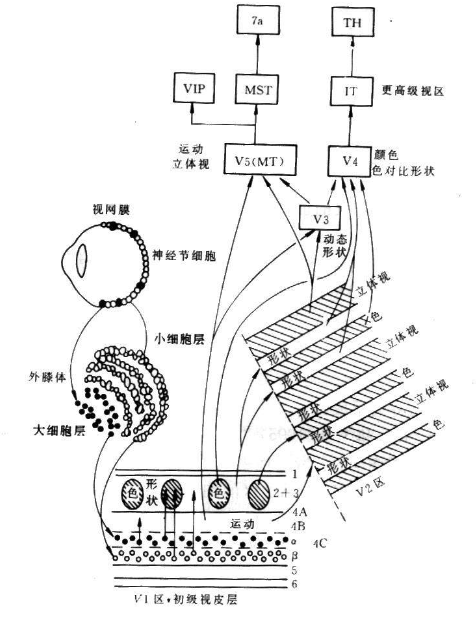
\includegraphics[width=0.8\textwidth]{picengchuanshu.png}
\caption{视觉传导示意图}\label{fig 10} 
\end{figure}




侧膝体(LGN)大细胞层的神经元直接投射到V1区皮层的4Cα层内,然后再依次投射到4B层的细胞,即形成“视网膜的M细胞(在图中M细胞用黑圆点表示)→LGN的大细胞层→4Cα→4B”的通路;另一方面,LGN的小细胞层的神经元则直接投射到V1区的4Cβ层内,然后再由4Cβ出发,分别投射到第2、3层内由细胞色素氧化酶染出的斑点和斑点间隙空间,即分成了两条通路:一条是“视网膜的P细胞(在图中P细胞用小圆圈表示)→LGN的小细胞层→4Cβ→斑点间隙区”。V1区的4B层无颜色选择性,但有方位选择性和运动方向选择性\cite{15:book}。另外,第2+3层的斑点内细胞也有可能接受来自4Cα层 的LGN大细胞的输入。可见,斑点内细胞和斑点间细胞行使着不同而又互补的功能:大多数斑点内细胞具有明显的颜色编码,对光谱的某种波长段的光刺激产生兴 奋,而对另一波长段的光刺激产生抑制,对方位无选择性;另有部分斑点内细胞为宽带细胞,对波长无选择性,却对亮度、对比度敏感。斑点间细胞则对方位有选择性,多数对颜色无选择性而对特定方位的线条或边界有反应,而不管其颜色如何;斑点间细胞虽无明显的颜色选择性,但仍能接受有颜色编码的LGN小细胞层神经元输入,因而对颜色仍有一定反应。由此看来,通过V1的加工产生了两个分离的细胞群:一群对方位无选择性但有明显的颜色编码(即有明显的颜色选择性),另一群无明显的颜色选择性但对方位有选择性\cite{14:misc}。
         


V2区深色窄条纹的皮层细胞接受V1区2+3层斑点内细胞的投射,它们没有方位选择性,约一半以上的细胞是颜色编码。V2区深色宽条纹内的细胞接受V1区4B层细胞的投射,它们没有颜色选择性,但绝大多数呈现方位选择性;它们最重要的性质是立体深度选择性,即对单眼刺激的反应很弱,而对双眼同时刺激的反应很强;对刺激在双眼水平位置上的变化(视网膜视差)非常敏感。在V2区亮 带内的皮层细胞接受V1区2+3层斑点间细胞的投射,它们具有方位选择性,但没有方向选择性;亮带内的皮层细胞与V1区斑点间细胞类似,也没有明显的颜色编码,但对颜色对比边界有反应。
        


由以上分析可见,在初级视皮层的V1、V2区内,通过串并存加工,颜色、形状、深度等不同视觉信息已经开始分离,下面会看到在V2以上的中高级视皮层,这种分离倾向会更为明显。
        


根据利文斯通、休伯和万·埃森等人\cite{14:misc}的研究成果,灵长目的中级视皮层加工的神经机制可用四个相对独立的子系统来说明:一个涉及运动,一个涉及颜色,两个涉及形状。
        


运动子系统在初级视皮层以外的中枢为V5区(也称MT区),其输入通路是“从视网膜的M细胞→LGN的大细胞层→V1区的4Cα→4B”,然后由4B再直接(或间接地经V2的深色宽条纹区)投射到V5区。
        


颜色子系统在初级视皮层以外的中枢为V4区,其输入通路是“从视网膜的P细胞→LGN的小细胞层→V1区的4Cβ→2+3层的斑点内细胞”,然后再直接(或间接地经V2的深色窄条纹区)投射到V4区。
        


其中一个形状子系统是以V4区为基础,它与颜色有关联。其输入通路是“从视网膜的P细胞→LGN的小细胞层→V1区的4Cβ→2+3层的斑点间细胞→V2的亮带区→V4”。另一个形状子系统是以V3区(19区)为基础,它侧重动态形状,即运动中的物体形状。其输入通路是“从M细胞→LGN的大细胞层→V1区的4Cα→4B”,然后由4B再直接(或间接地经由V2的深色宽条纹区)投射到V3。
        


迄今为止,我们只讨论了由初级视皮层V1、V2区向更高级视皮层区(如 V3、V4、V5)的“前向投射”(或“正向投射”),是否也存在更高级视皮层区向V1、V2的“反向投射”呢?根据万·埃森等人对猕猴大脑所进行的大量神经生理实验表明,这种反向投射不仅存在,而且几乎都是往返的,除了个别例外,一般都是双向交互投射,即反向投射几乎和正向投射一样多。例如V1 和V2、V3、V4、V5(MT区)之间存在双向交互投射,V5至少和七个确定的视皮层区存在交互投射:MST区(内侧上颞区)、VIP区(腹内顶区)、VP区(腹后区)、V4区、V3区、V2区和V1区,其中MST和VIP属于更高级的视区。
         


虽然在解剖学上已有反向投射的大量证据,但是目前对中、高级视皮层向低级视皮层反向投射(信息从高层向低层反馈输入)的意义、作用还了解得很不够\cite{14:misc}。值得注意的是,低级视皮层的V1与V2区各亚层内细胞的分工比较明确,而从更高级视皮层返回到V1和V2的投射则是弥散的。以V1区的4B层为例,4B的细胞不仅投射到V5而且投射到V3区和V2的细胞色素氧化酶染色的宽条纹区,这些区均有返回性弥散投射。这样,V5就可以通过这些途径返回到V1区的4B亚层并对V3区和V2的宽条纹区产生影响,从而使主管运动信息的4B-V5与主管形状信息的V3之间发生整合作用。同样,V5和V4对V2的反向投射也是弥散性的,即V2区中的宽条纹区、窄条纹区和亮带都有来自V5、V4的投射,因此一方面V5可以通过对V3的反向投射以及V3对V4的正向投射影响V2窄条纹区内的颜色信息处理;另方面,主管颜色信息处理的V4通过对V3的反向投射以及V3对V2宽条纹区的反向投射,也可以影响运动和动态形状的信息处理。可见,返回性的“反馈”信息通路不仅返回到原有视区输入神经元所在的亚层,而且分布到整个初级视区,从而使颜色、形状和运动等信息彼此联系起来,起到了整合的作用。


\section{总结}



人类和高级哺乳动物对世界的物体的认知能力是无穷的\cite{15:book},这就要求视觉系统具有极高的处理和组合能力,把视觉传导既平行又序列的进行处理过的亮度、形状、颜色、运动方向、运动速度、深度等各种视觉信息整合起来,形成完整的视知觉,从而感知世界。
        

根据以上对视网膜、外膝体和视皮层的综述,我们可以看到视觉信息处理机制是既平行又分级串行的信息处理机制\cite{16:book}。视觉系统组织成不同的通路对视觉信息的不同侧面进行传递和处理,它们相互协作,共同组成了完整的视觉感知系统。
        


视觉信息处理的研究也面临着严峻的挑战,一个根本的问题在于脑的各部分越来越趋向于分工处理各种各样的视觉特征,而我们的视觉和认知过程却又把这些各种各样的视觉特征综合成一个完整的视觉实体\cite{17:book}。随着神经生物学的发展,视觉传导神经通路和视觉信息处理的研究还将进一步深入。本综述还存在很多不足的地方需要进一步改进,并且它将随着科学的发展而不断的进行完善。

\bibliographystyle{plain}
\bibliography{visual_trans}


\end{document}
